
\documentclass[twoside]{article}
\usepackage{CJKutf8}

%\usepackage{graphics}
\usepackage{graphics}
\usepackage{geometry}
\usepackage{forest,amsmath}
\usepackage{enumerate}
\usepackage{url}
\usepackage{latexsym,bm,amssymb}

\geometry{left=2.5cm,right=2cm,top=2.5cm,bottom=2.5cm}

%\setlength{\oddsidemargin}{0.25 in}
%\setlength{\evensidemargin}{-0.25 in}
%\setlength{\topmargin}{-0.6 in}
%\setlength{\textwidth}{6.5 in}
%\setlength{\textheight}{8.5 in}
%\setlength{\headsep}{0.75 in}
\setlength{\parindent}{0 in}
\setlength{\parskip}{0.1 in}

\usepackage{listings}
\usepackage{color}
\renewcommand\lstlistingname{Quelltext} % Change language of section name
\lstset{ % General setup for the package
    language= C,
    %basicstyle=\small\sffamily,
    basicstyle=\ttfamily,
    numbers=left,
     numberstyle=\tiny,
    frame=tb,
    tabsize=4,
    columns=fixed,
    showstringspaces=false,
    showtabs=false,
    keepspaces,
    commentstyle=\color{red},
    keywordstyle=\color{blue}
}

%
% The following commands set up the lecnum (lecture number)
% counter and make various numbering schemes work relative
% to the lecture number.
%
%\newcounter{lecnum}
%\renewcommand{\thepage}{\thelecnum-\arabic{page}}
%\renewcommand{\thesection}{\thelecnum.\arabic{section}}
%\renewcommand{\theequation}{\thelecnum.\arabic{equation}}
%\renewcommand{\thefigure}{\thelecnum.\arabic{figure}}
%\renewcommand{\thetable}{\thelecnum.\arabic{table}}

%
% The following macro is used to generate the header.
%


%


%Use this command for a figure; it puts a figure in wherever you want it.
%usage: 
%\begin{figure}
%\begin{center}
%\includegraphics[width=5in]{fig-file}
%\caption{}\label{fig:delavl}
%\end{center}
%\end{figure}

%%% Use the following command for a table
%%%

% Use these for theorems, lemmas, proofs, etc.
\newtheorem{theorem}{Theorem}[theorem]
\newtheorem{lemma}[theorem]{Lemma}
\newtheorem{proposition}[theorem]{Proposition}
\newtheorem{claim}[theorem]{Claim}
\newtheorem{corollary}[theorem]{Corollary}
\newtheorem{definition}[theorem]{Definition}
\newenvironment{proof}{{\bf Proof:}}{\hfill\rule{2mm}{2mm}}

% **** IF YOU WANT TO DEFINE ADDITIONAL MACROS FOR YOURSELF, PUT THEM HERE:

\begin{document}
\begin{CJK*}{UTF8}{gbsn}
	%FILL IN THE RIGHT INFO.
	%\lecture{**LECTURE-NUMBER**}{**DATE**}{**LECTURER**}{**SCRIBE**}
	%\lecture{1}{Project Name}{Deshi Ye}{Student 1, Student 2, 学生3}
	%\footnotetext{These notes are partially based on those of Nigel Mansell.}
	\title{Flexible}
	\date{}
	%\maketitle
	% **** YOUR NOTES GO HERE:

	% Some general latex examples and examples making use of the
	% macros follow.  
	%**** IN GENERAL, BE BRIEF. LONG SCRIBE NOTES, NO MATTER HOW WELL WRITTEN,
	%**** ARE NEVER READ BY ANYBODY.
	\section{Introduction}
	In this program, we decide to implement the Flappy game with LC-3 assembly language. In the original game, a bird is flying from left to right, but in this game, it may fly from top to bottom. In the game, the bird is represented by 3 continuous letters(for example $aaa$). Without control, it will fall to left, but the user can make it fly to right by 1-9 blocks (chars) by clicking corresponding numbers. By the way, the bird will change its appearance after the user clicked a-z.
	
	In this program, falling to gound (the leftmost side) won't end the game. And flying too high (right) is not allowed,we just put the bird on the rightmost side if it fly too high.
	
	Here is an example:\\
	.....aaa............ User Input(you don't need to print)\\ ....aaa............. \\...aaa..............\\ ............aaa..... <-9\\ ...........aaa...... \\.................aaa <-8\\ ................aaa. \\...............aaa.. \\..............aaa...\\ .............aaa....\\ ............aaa.....\\ ...........aaa...... \\..........aaa....... \\.........aaa........\\ ........ddd......... <-d\\ .......ddd..........\\ ......ddd...........\\ .....ddd............ \\....ddd.............\\ ...ddd.............. \\..aaa............... <-a \\.aaa................\\ aaa.................\\ aaa................. \\ooo................. <-o\\ ooo.................\\ ....ooo............. <-4\\ ...ooo..............\\
	
	\section{Algorithm Specification}
	The program can be roughly divided into two part: the interrupt function and the main function
	
	In order to motivate the interrupt, we should initialize the KBSR[14] when initializing the program. So we rewrite the instructions from x0200. In the new instructions, we add a instruction to load x4000 to KBSR, so that the KBSR[14] will be 1. In this way, when we press the keyboard, the KBSR will create a INT signal to interrupt the program and the PC will change to the content of x0180. We also load the address of interrupt function to x0180, which is x2000. When we press the keyboard, the KBSR[15] will be 1, INT signal gengerated, then the PC will come to x2000, where the interrupt function locates.
	
	To handle the problem that the player inputs multiple operation one times. We use a data structure to store the operations inputted. A queue is a good choice. When a character is inputted, we just store it into the queue. When the main function ready to output, we just take out the data in queue and analyse them.
	
	After complex introduction, next is the detail of interrupt function and the main function.
	
	In interrupt function, we initially check the KBSR[15]. when it's 1, we take the KBDR into register and then enqueue it into queue.
	
	\begin{lstlisting}[mathescape=true]
		while KBSR[15] != 1
			loop
		R0 $\leftarrow$ KBDR
		enqueue(R0)
	\end{lstlisting}
	
	In main function, we firstly use a loop to cause the delay. After the loop, the program dequeues the data in the queue with checking whether they are characters or digit. If a data is characters, the name of bird will be changed. If the data is a digit otherwise, we change the ascii code into digit and add it with the height. Finally, before print out, we should check whether the height is overflow or underflow and do some adjustments to it.
	
	\begin{lstlisting}[mathescape=true]
		count $\leftarrow$ x6000
		R1 $\leftarrow$ height
		while count > 0
		 	count--
		 c $\leftarrow$ dequeue
		 while c != -1
		 	if c is character
		 		name $\leftarrow$ c
		 	if c is digit
		 		R1 $\leftarrow$  R1 + c - '0'
		 if R1 == height
		 	R1 $\leftarrow$ R1 - 1
		 print(name, height)
	\end{lstlisting}


	About the function to output according to name an height, it firstly print `·' as much as the height. Then, the program output three characters of the name. Finally, we calculate $17-height$ and output `·' as much as it.
	\begin{lstlisting}[mathescape=true]
		for i = 1 to height
			R0 $\leftarrow$ '·'
			trap x21
		R0 $\leftarrow$ name
		trap x21
		trap x21
		trap x21
		height $\leftarrow$ 17 - height
		for i = 1 to height
			R0 $\leftarrow$ '·'
			trap x21
	\end{lstlisting}
	
	
	Next is the implement of the data structure, which is a queue supporting the operation of dequeue and enqueue. It's much like the data structure in Lab3, so we don't explain much about it.
	
	\begin{lstlisting}[mathescape=true]
		enqueue: R0 is the element , front_ptr is the point to the front of queue
		*(--front_ptr) $\leftarrow$ R0
	\end{lstlisting}


	\begin{lstlisting}[mathescape=true]
		dequeue: front_ptr is the point to the front of queue,
			back_ptr is the point to the back of queue
		if front_ptr == back_ptr + 1
			R0 $\leftarrow$ -1
		else 
			R0 $\leftarrow$ *(back_ptr--)
	\end{lstlisting}


	\section{Q and A}
	\begin{itemize}
		\item 	Q: what you put in each part of your program ?
		
				A: The code of the program is mainly constructed by three parts. First one is from x0200, where we should do some initialization. We initialize the interrupt function address of x0180, and set the KBSR[14] to be 1. Second one is from x2000, where the keyboard interrupt function locates. Here, we read the character in KBDR and store it into queue. Third one is from x3000, which is the main function. We form a loop and the dequeue the item in queue until the queue becomes empty. After getting an item, we check whether it is character or digit, then do operations to name or height. Finally we output a line according to name and height.
	\end{itemize}


	\section{essential parts of code}
	Fig 1 is the implement of code from x0200
	\begin{figure}[htbp]
		\small
		\centering
		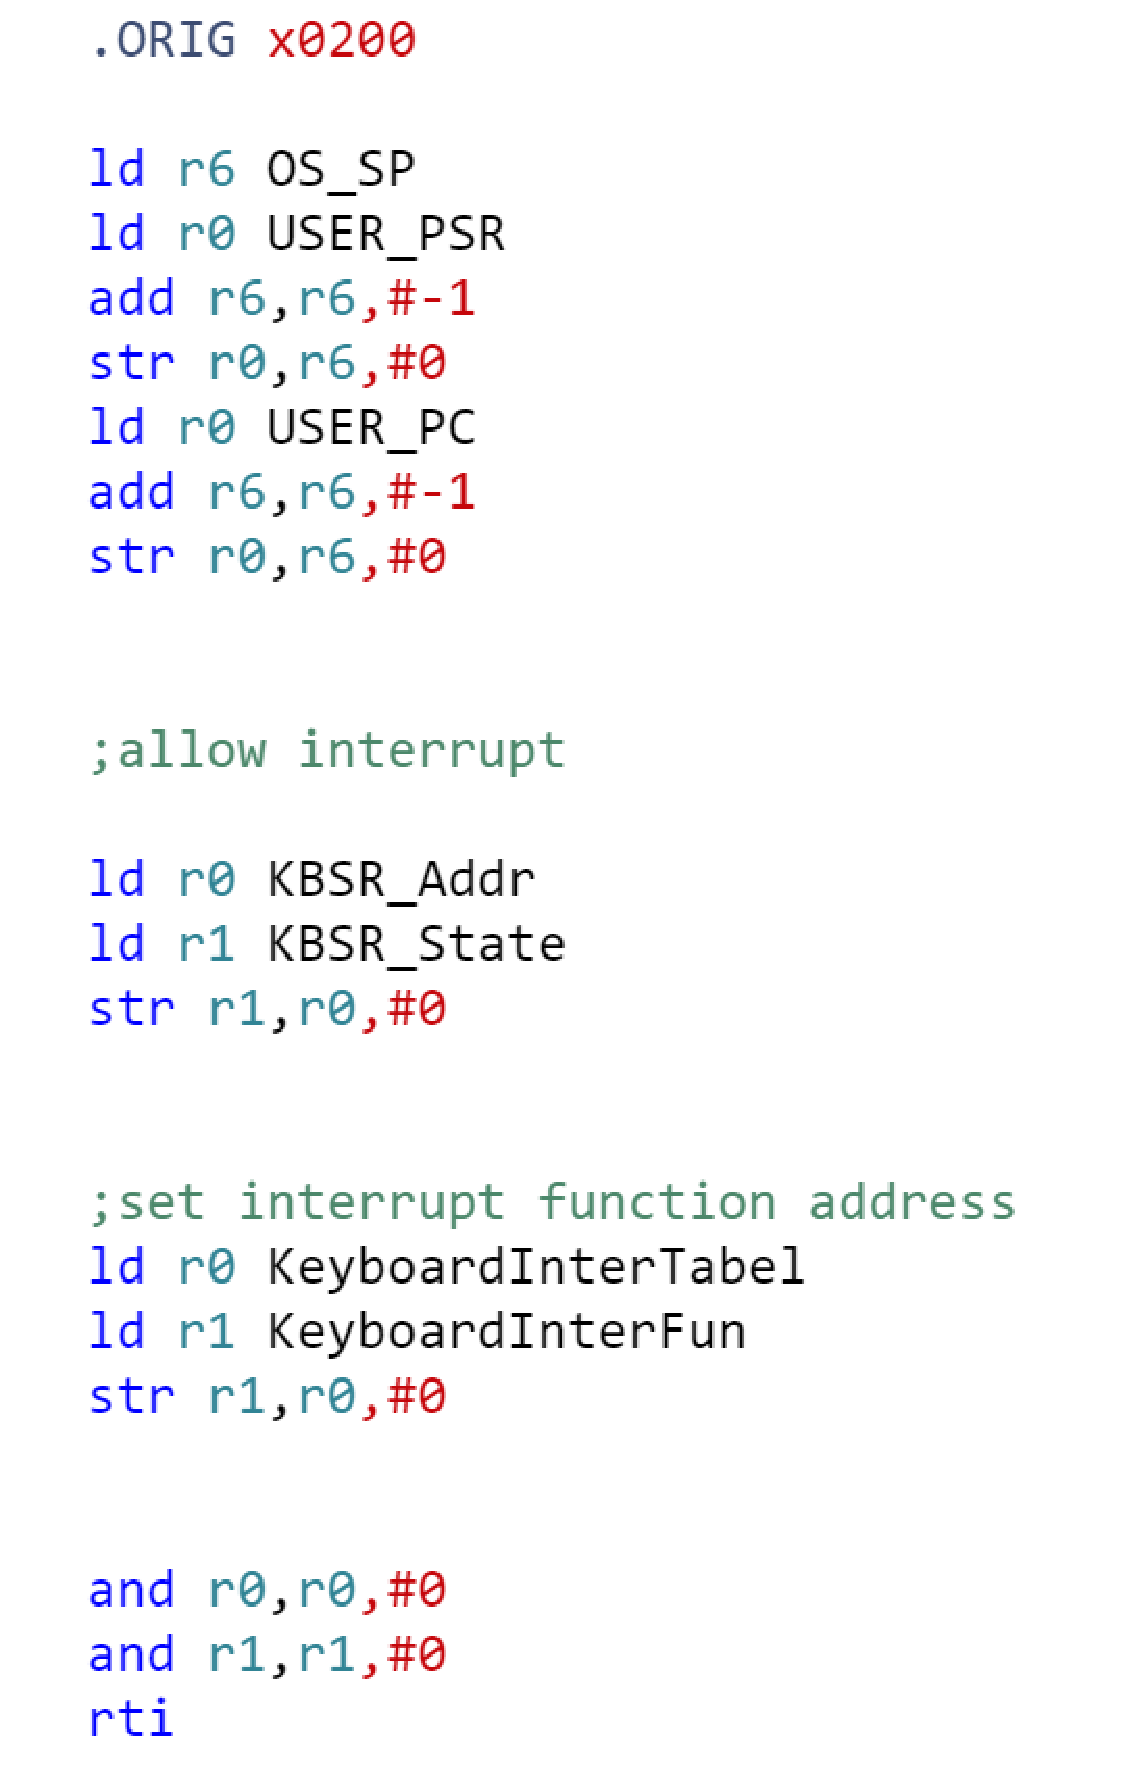
\includegraphics[width=0.4\textwidth]{fig1.eps}
		\caption{Fig 1} %名字
	\end{figure}


	Fig 2 is the implement of code from x2000
	\begin{figure}[htbp]
		\small
		\centering
		\includegraphics[width=0.7\textwidth]{fig2.eps}
		\caption{Fig 2} %名字
	\end{figure}

	Fig 2 is the main function from x3000

	\begin{figure}[htbp]
		\centering
		\caption{Fig 3} %名字
		\begin{minipage}[t]{0.4\textwidth}
			\small
			\centering
			\includegraphics[width=0.9\textwidth]{fig3.eps}
		\end{minipage}
		\begin{minipage}[t]{0.4\textwidth}
			\small
			\centering
			\includegraphics[width=0.9\textwidth]{fig4.eps}
		\end{minipage}
		
	\end{figure}
	
	
	
	Fig 4 is the implement of getdata function

	\begin{figure}[htbp]
		\centering
		\caption{Fig 4} %名字
		\begin{minipage}[t]{0.4\textwidth}
			\small
			\centering
			\includegraphics[width=0.9\textwidth]{fig5.eps}
		\end{minipage}
		\begin{minipage}[t]{0.4\textwidth}
			\small
			\centering
			\includegraphics[width=0.9\textwidth]{fig6.eps}
		\end{minipage}
		\begin{minipage}[t]{0.4\textwidth}
			\small
			\centering
			\includegraphics[width=0.9\textwidth]{fig7.eps}
		\end{minipage}
		
	\end{figure}


\end{CJK*}
\end{document}





